\chapter{Potentiel électrique}


\section{Énergie potentielle électrique}

\marginnote{
  Tremblay \S 4.1

  Lafrance \S 4.1
}

\minisec{Objectif}

\begin{enumerate}
  \item L'étudiant pourra calculer le travail fait par une force électrique.
  \item L'étudiant saura comment démontrer que la force électrique est une
    force conservative.
  \item L'étudiant pourra calculer l'énergie potentielle électrique et sera en
    mesure d'expliquer le lien entre la force et l'énergie potentielle.
\end{enumerate}



\begin{diapobox}
\minisec{Exercice de rappel sur la notion de travail}

Classez les situations suivantes en ordre croissant du travail fait par la
force électrique sur la charge $q > 0$.

\begin{center}
  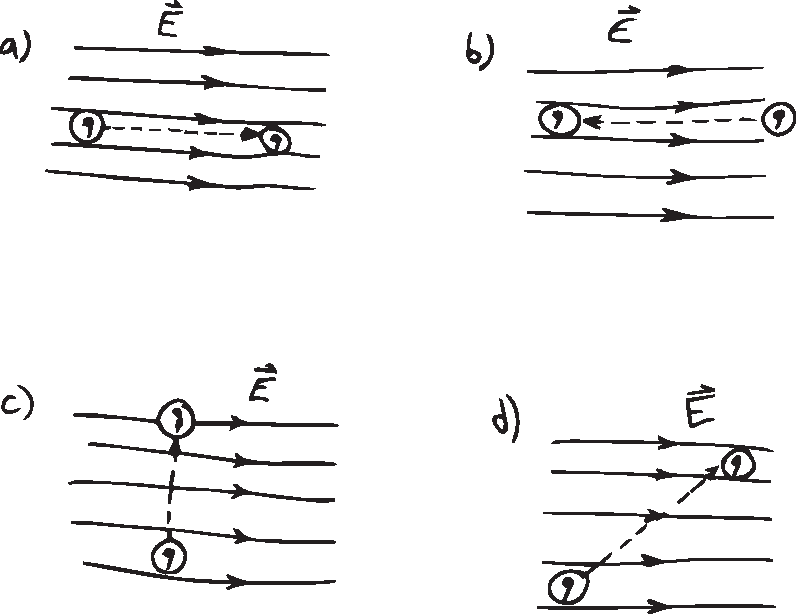
\includegraphics[scale=0.7]{04-potentiel/figures/travail-force-electrique.pdf}
\end{center}

\textit{Solution}: $W_b < W_c < W_a = W_d$
\end{diapobox}

\clearpage

\minisec{Le travail fait par une force électrique}

\begin{fondamentalbox}
Si une particule se déplace du point $A$ au point $B$, le travail
effectué par une force est
\[
  W \equiv \int_A^B \vec{F} \cdot d\vec{s}
\]
où $d\vec{s}$ est une petite partie du chemin parcouru. 
\end{fondamentalbox}
Dans le cas simple où la trajectoire est une ligne droite de longueur $L$ et la
force est constante
\[
  W = FL.
\]
On considère une région d'espace avec un champ électrique $\vec{E}$. Une charge
ponctuelle $q$ dans cette région subit une force électrique $\vec{F} =
q\vec{E}$. 
On peut récrire l'expression du travail en terme du champ électrique
\[
  W = q \int_A^B \vec{E}\cdot d\vec{s}
\]
\begin{center}
  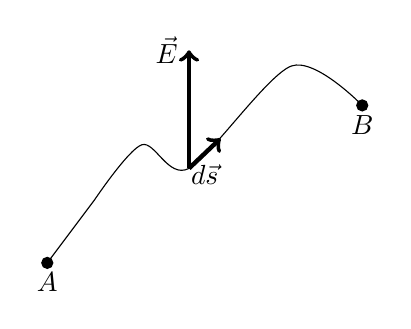
\begin{tikzpicture}
    \coordinate (A) at (0, 0);
    \coordinate (B) at (4, 2);
    \draw[fill=black] (A) circle (2pt);
    \draw[fill=black] (B) circle (2pt);
    \node[below] (nA) at (A) {$A$};
    \node[below] (nB) at (B) {$B$};
    \draw (A) -- plot[smooth] coordinates {(0.6, 0.8) (1.2, 1.5) (1.8, 1.2) (3.1, 2.5) (B)};
    \draw[ultra thick, ->] (1.8, 1.2) -- node[below] {$d\vec{s}$} (2.2, 1.58);
    \draw[ultra thick, ->] (1.8, 1.2) -- ++(0, 1.5) node[left] {$\vec{E}$};
  \end{tikzpicture}
\end{center}


\minisec{La force électrique est conservative}

On peut montrer que le travail fait par la force électrique est indépendante du
chemin suivi pour aller du point $A$ au point $B$. Vous avez vu le même genre
de résultat pour la force gravitationnelle. Par opposition, le travail fait par
le frottement est dépendant du chemin.

Une force pour laquelle le travail est indépendant du chemin est
\textbf{conservative}.

Rappelez-vous le cas de la force gravitationnelle à la surface de la Terre
(avec l'axe $y$ qui pointe vers le haut)
$$W_g = -mg \Delta y$$


\minisec{Énergie potentielle électrique}

Puisque la force électrique est conservative, on peut lui associer une énergie
potentielle. On définit l'énergie potentielle électrique de la même façon que
nous avons défini l'énergie potentielle gravitationnelle: c'est l'opposé du
travail fait par la force,
$$\Delta U \equiv -W$$
c'est-à-dire,
\[
  \Delta U = - q\int_A^B \vec{E} \cdot d\vec{s}
\]


\begin{diapobox}
  \minisec{Exercice}

  Une particule de charge \SI{-8.00}{\micro\coulomb} est placée
  \SI{2.00}{\meter} à gauche d'une grande plaque verticale portant une charge
  surfacique de \SI{50.0}{\nano\coulomb\per\meter\squared}. La particule
  s'approche de \SI{1.00}{\meter} de la plaque.

  \marginnote{
    \begin{center}
      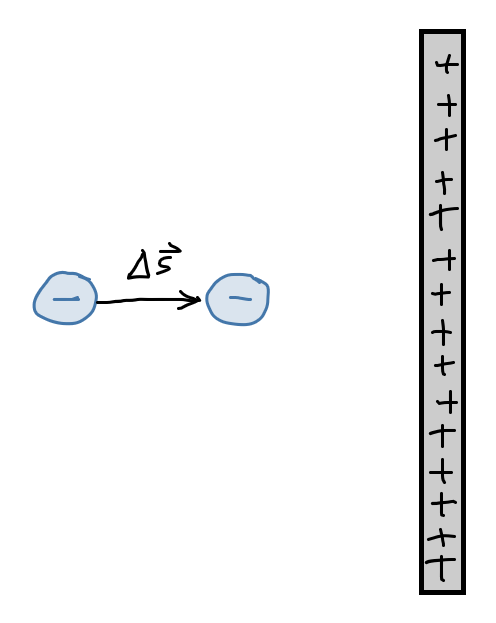
\includegraphics[width=0.3\textwidth]{04-potentiel/figures/charge_neg_gauche_plaque.png}
    \end{center}
  }

  Quel est le travail effectué par la force électrique?

  Quel est la variation d'énergie potentielle électrique?

  Si aucun travail externe n'est effectué et que la particule était
  initialement au repos,
  quelle est la vitesse de la particule à la fin de son mouvement?
\end{diapobox}

\begin{reponsebox}
  Le champ produit par la plaque a une grandeur $E = \sigma / 2\varepsilon_0$
  et est orienté vers la droite. Le travail produit par la force électrique est
  donc
  \begin{align*}
    W &= q\int_{\SI{0}{m}}^{\SI{1}{m}} \vE \cdot d\vec{s}  \\
      &= -qE \int_{\SI{0}{m}}^{\SI{1}{m}} ds \\
      &= -qEL  \\
      &= \SI{22.59}{\milli\joule}
  \end{align*}

  L'énergie potentielle électrique a donc diminuée de \SI{22.59}{\milli\joule}.

  Par le principe de conservation de l'énergie, l'énergie cinétique a augmenté
  de \SI{22.59}{\milli\joule}. Puisque l'énergie cinétique initiale était
  nulle, on a donc que la vitesse à la fin est
  \begin{align*}
    v_f &= \sqrt{\frac{2 K_f}{m}}  \\
        &= \SI{475.3}{\meter\per\second}
  \end{align*}
  vers la droite.
\end{reponsebox}


\begin{diapobox}
  Un atome d'hydrogène est constitué d'un électron et d'un proton. On
  assemble un atome d'hydrogène à partir d'un électron et d'un proton isolé
  qu'on approche jusqu'à une distance de \SI{1.06e-10}{\meter}. Si on pose que
  l'énergie potentielle du système est nulle lorsque les deux particules sont
  isolées, quelle est l'énergie potentielle de l'atome d'hydrogène assemblé?
  \marginnote{
    \begin{center}
      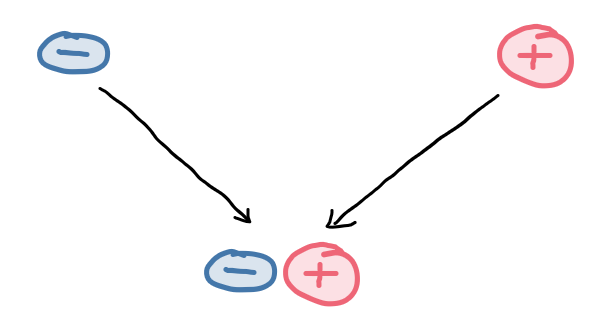
\includegraphics[width=0.3\textwidth]{04-potentiel/figures/hydrogene.png}
    \end{center}
  }[-4\baselineskip]
\end{diapobox}

\begin{reponsebox}
  On place le proton à l'origine. L'électron est à l'infini. La force
  électrique sur l'électron est donnée par la loi de Coulomb
  \begin{align*}
    \vF &= -\frac{ke^2}{r^2} \vu_r
  \end{align*}
  Le travail fait par la force électrique est
  \begin{align*}
    W &= \int_\infty^a \vF \cdot d\vec{r}  \\
      &= -ke^2 \int_\infty^a \frac{dr}{r^2} \\
      &= -ke^2 \left[ \frac{-1}{r} \right]_\infty^a  \\
      &= -ke^2 \left( \frac{-1}{a} - \frac{-1}{\infty} \right)  \\
      &= \frac{ke^2}{a}  \\
      &= \SI{2.156e-18}{\joule}
  \end{align*}
  Le changement d'énergie potentielle est $\Delta U = -W =
  -\SI{2.156e-18}{\joule}$. L'énergie potentielle au début est
  nulle, alors l'énergie potentielle finale est $-\SI{2.156e-18}{\joule}$.
\end{reponsebox}


%\minisec{Exemple}

%\marginnote{40 minutes}

%On considère une mince tige métallique cylindrique très longue portant une
%charge uniforme.  La densité linéique de charge est de $\lambda =
%\SI{0.948}{\micro\coulomb\per\meter}$. Un électron est relâché \SI{35}{mm}
%de la tige.

%\begin{enumerate}
  %\item Calculer la variation d'énergie potentielle du système après que
    %l'électron se soit déplacé de \SI{1}{cm}.
  %\item Si l'électron était initialement au repos, déterminer sa vitesse à la
    %fin de son déplacement.
  %\item Tracer un graphique du module du champ électrique généré par la tige en
    %fonction de la distance par rapport à son axe.
  %\item Tracer un graphique de l'énergie potentielle de l'électron en fonction
    %de sa distance par rapport à l'axe de la tige.
%\end{enumerate}

%\paragraph{Solution}

%\begin{center}
  %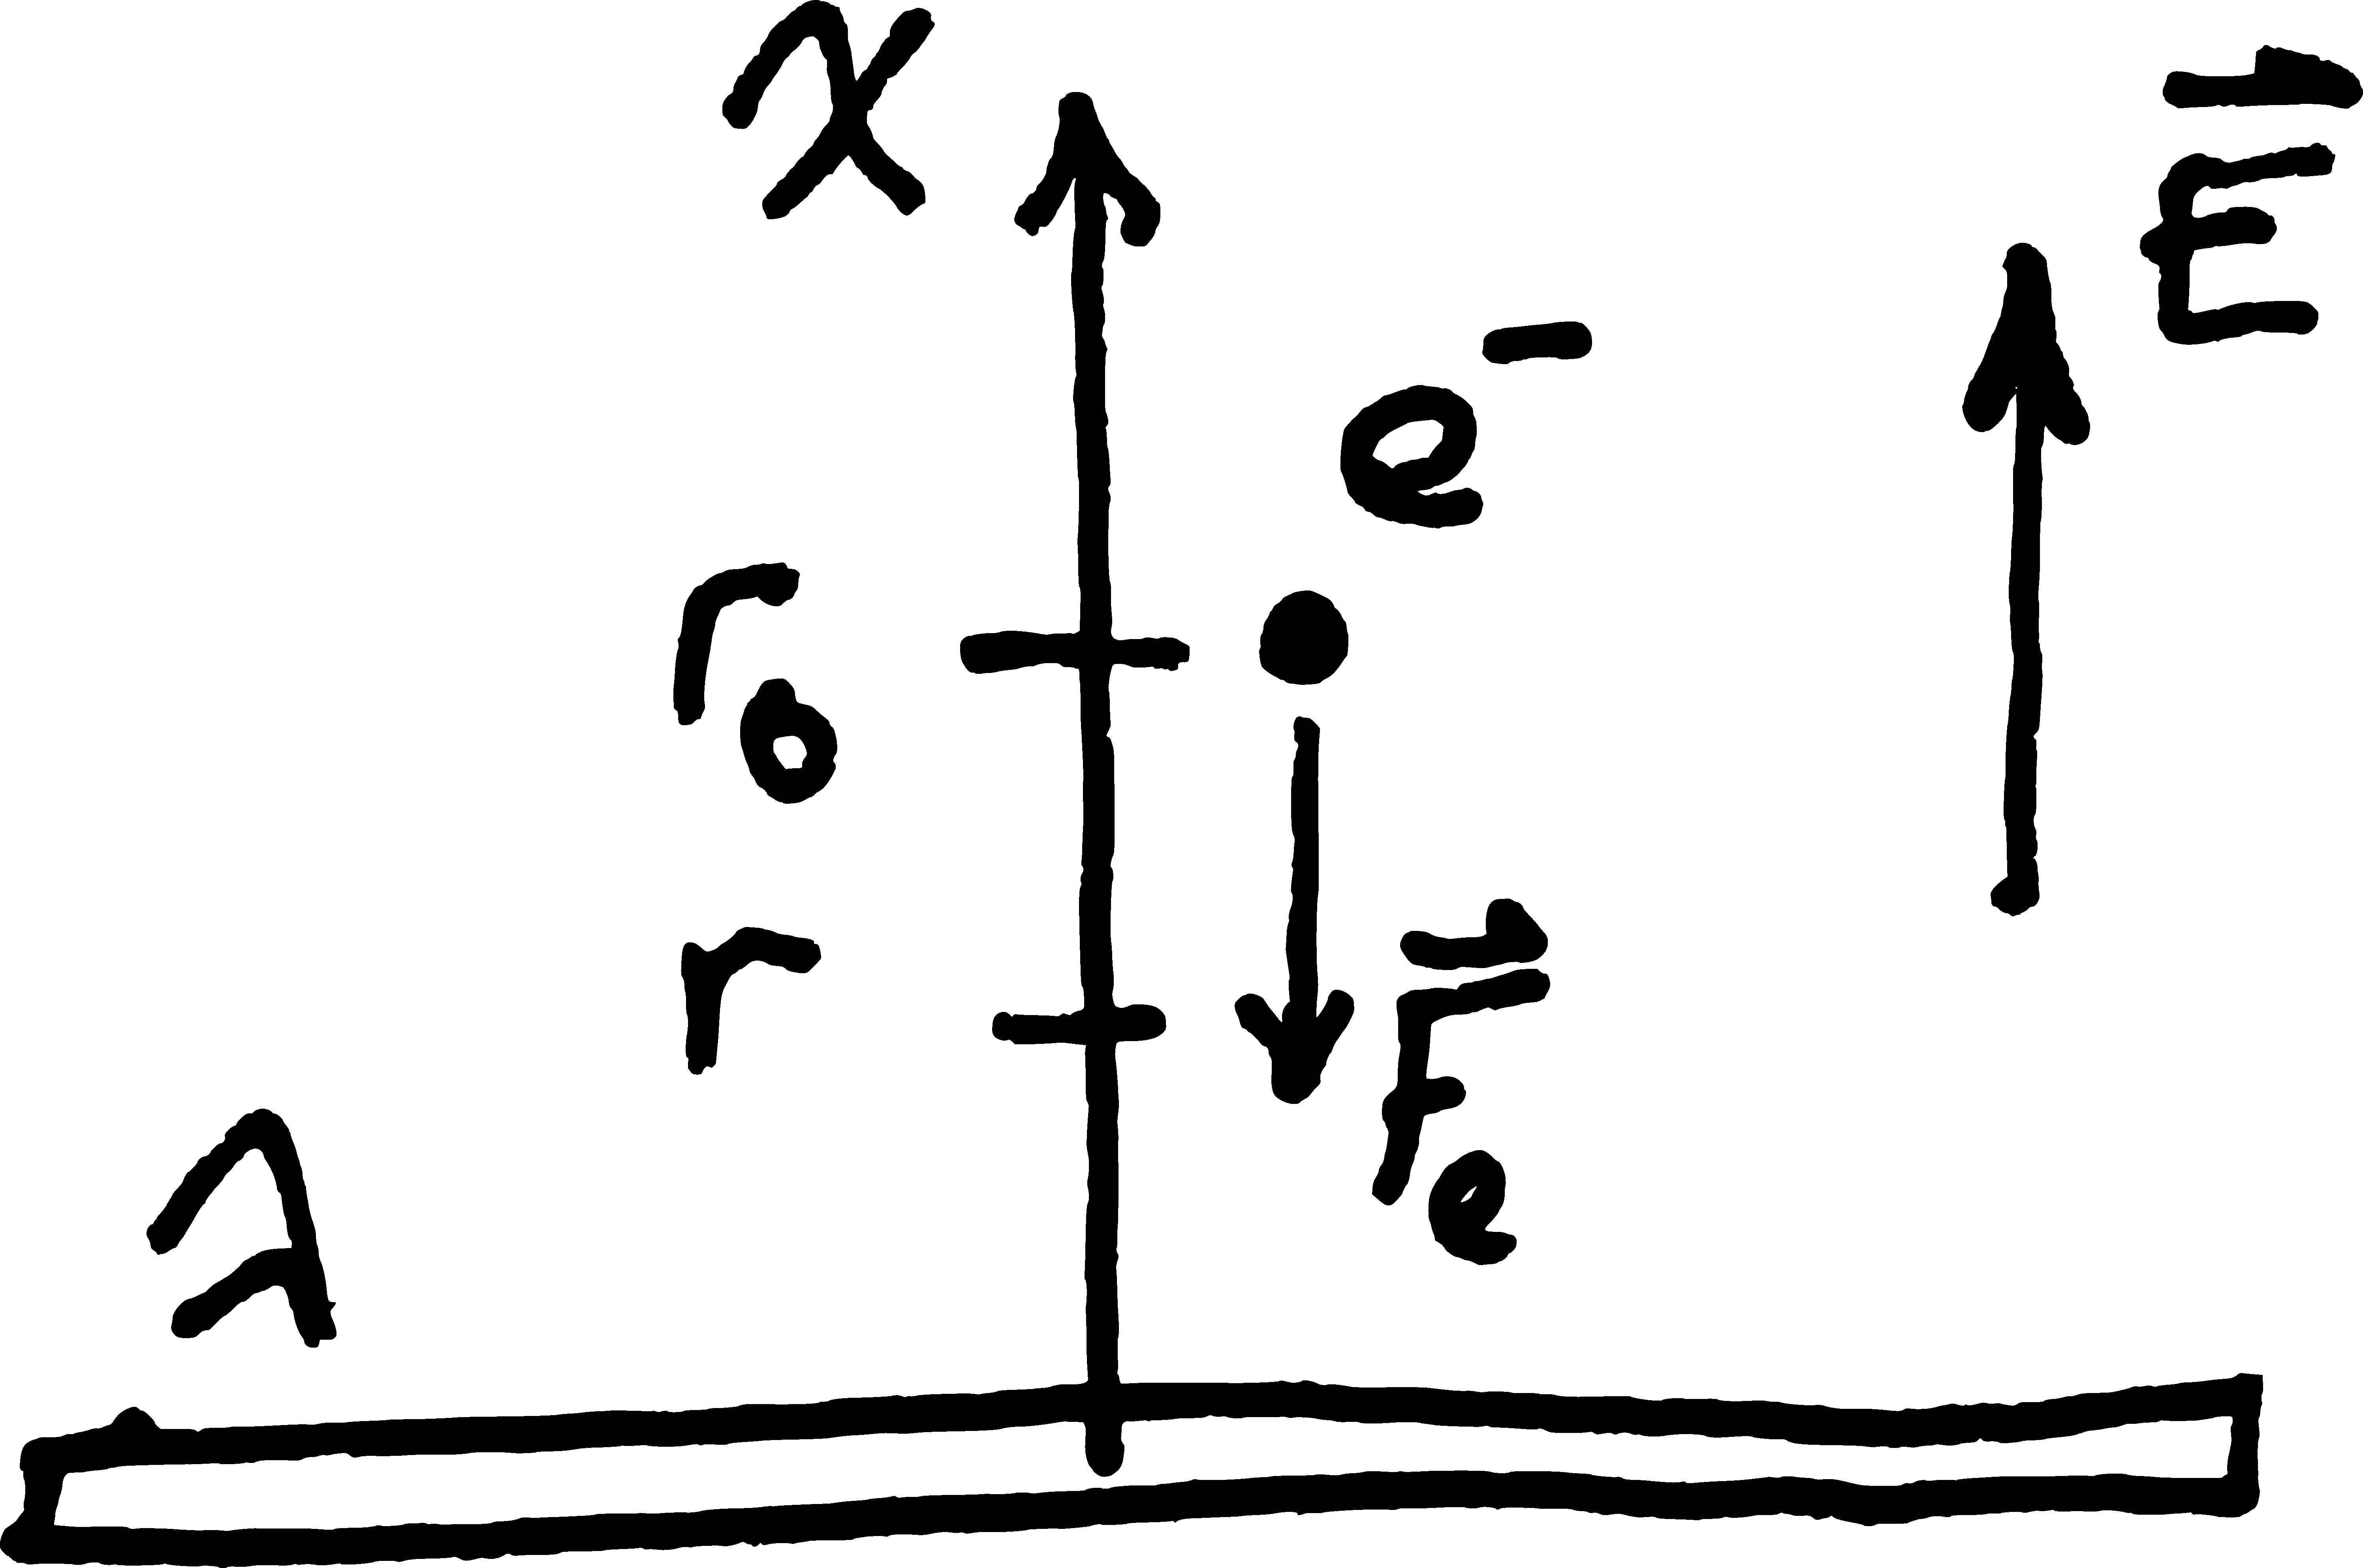
\includegraphics[scale=0.04]{04-potentiel/figures/exercice-tige-energie-potentielle.pdf}
%\end{center}
%\begin{enumerate}
    %\item L'électron est attiré par la tige chargée positivement, donc il se
        %rapproche de la tige. Le champ électrique de la tige est celui d'un fil
        %infini soit
        %\[\vE = \frac{2k\lambda}{x} \xhat.\]
        %On peut donc calculer la différence d'énergie potentielle
        %\begin{align*}
            %\Delta U &= -q \int_{r_0}^{r} \frac{2k\lambda}{x} \xhat \cdot d\vec{s} \\
                     %&= -2k\lambda q \int_{r_0}^r \frac{1}{x} \xhat \cdot (dx \xhat
                        %+ dy \yhat + dz \zhat) \\
                     %&= -2k\lambda q \int_{r_0}^r \frac{1}{x} dx \\
                     %&= -2k\lambda q \left[ \ln(r) - \ln(r_0) \right] \\
                     %&= -2k\lambda q \ln\left( \frac{r}{r_0} \right) \\
                     %&= 2k\lambda e  \ln\left( \frac{r}{r_0} \right) \\
                     %&= \SI{-9.186e-16}{J}
        %\end{align*}
    %\item Au départ, son énergie cinétique était nulle car il était immobile,
        %par conséquent
        %\begin{align*}
            %\Delta K = K_f - K_i = K_f.
        %\end{align*}
        %Par le principe de conservation de l'énergie mécanique
        %\begin{align*}
            %\Delta K + \Delta U &= 0 \\
            %\Delta K &= -\Delta U \\
            %\frac{1}{2} m_e v^2 &= -\Delta U \\
            %v &= \sqrt{\frac{-2\Delta U}{m_e}} \\
            %v &= \SI{4.491e7}{m/s}
        %\end{align*}
        %Donc
        %\[\vec{v} = -\SI{4.491e7}{m/s} \xhat\]
    %\item Les graphiques du module du champ magnétique et de l'énergie
        %potentielle sont ci-dessous.

      %\begin{center}
        %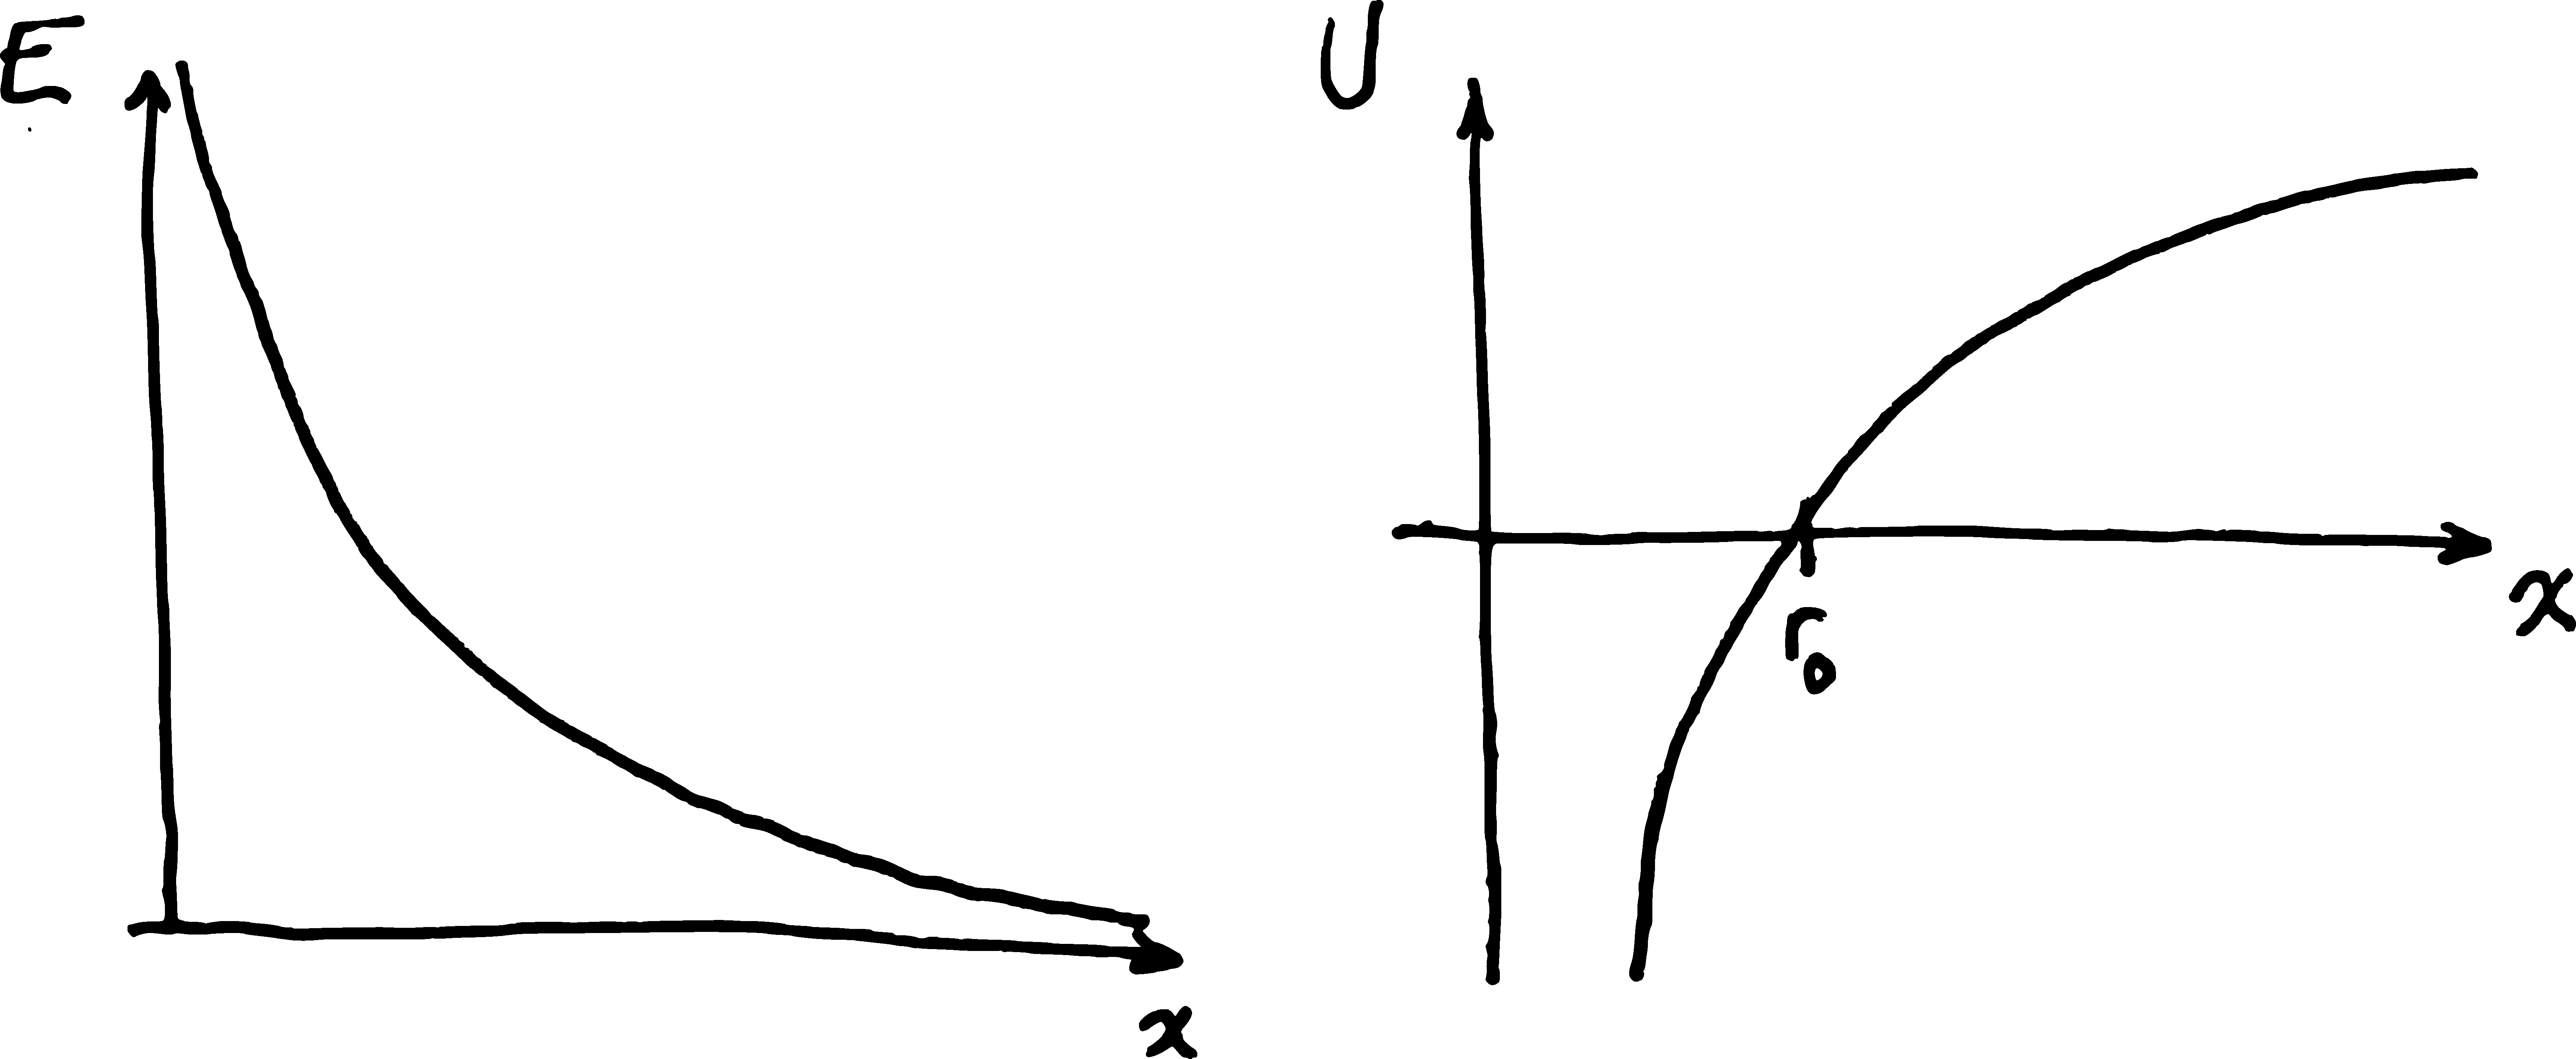
\includegraphics[scale=0.09]{04-potentiel/figures/exercice-tige-energie-potentielle-graphiques.pdf}
      %\end{center}
%\end{enumerate}



\section{Potentiel électrique}

\marginnote{
  Tremblay \S 4.2

  Lafrance \S 4.2
}

\minisec{Objectif}

\begin{enumerate}
  \item L'étudiant comprendra les concepts de potentiel électrique et de
    différence de potentiel. Il pourra expliquer le lien entre le potentiel et
    le champ électrique.
\end{enumerate}



Dans la formule pour l'énergie potentielle électrique
\[
  \Delta U = -q \int_A^B \vec{E}\cdot d\vec{s},
\]
on remarque que l'intégrale ne dépend pas du tout de la charge qui se déplace.
L'intégrale dépend uniquement de la source du champ électrique. Comme nous
l'avions fait avec la force et le champ électrique, nous pouvons définir une
quantité qui ne dépend que de la source
\[
  \Delta V = - \int_A^B \vec{E}\cdot d\vec{s}.
\]
Cette quantité s'appelle une \textbf{différence de potentiel électrique}.
C'est l'énergie potentielle par unité de charge
\[
  \Delta V \equiv \frac{\Delta U}{q}
\]
À chaque point de l'espace on peut assigner une valeur de \textbf{potentiel
  électrique} définie de telle sorte que $\Delta V = V_B - V_A$.

Les unités de la différence de potentiel sont les volts
$$\SI{1}{V} = \SI{1}{Nm/C}$$
On exprime souvent le champ électrique en \si{\volt\per\meter}.

Si une particule chargée $q$ se déplace entre deux points séparés par une
différence de potentiel $\Delta V$, sont énergie potentielle varie de
\[
  \Delta U = q \Delta V
\]


\begin{diapobox}
  \minisec{Électron entre des plaques}

  Deux grandes plaques métalliques sont maintenues à une différence de potentiel
  de \SI{12}{V}. Elles sont séparées d'une distance de \SI{1}{cm}. Un électron
  qui se trouve juste à côté d'une des plaques se déplace jusqu'à l'autre plaque.
  Si l'électron est initialement immobile, déterminer le module de sa vitesse
  lorsqu'il atteint l'autre plaque.

  \begin{center}
    \begin{tikzpicture}
      \draw[very thick] (0, 0) -- (0, 2);
      \draw[very thick] (4, 0) -- (4, 2);
      \foreach \y in {0.25, 0.75, ..., 1.9} {
        \node at (-0.3, \y) {$+$};
        \node at (4.3, \y) {$-$};
      }
      \fill (3.8, 1) circle (0.1);
      \node at (3.75, 0.6) {$e^{-}$};
      \draw[->] (3.65, 1) -- ++(-1, 0);
    \end{tikzpicture}
  \end{center}
\end{diapobox}

\begin{reponsebox}
L'énergie cinétique initiale est de $0$ car l'électron est au repos. La
variation d'énergie potentielle lorsque l'électron passe de la plaque négative
à la plaque positive est de
\begin{align*}
  \Delta U &= q \Delta V \\
           &= -e \Delta V
\end{align*}
où $\Delta V = \SI{12}{V}$. Par le principe de conservation de l'énergie
mécanique, on a
\begin{align*}
  \Delta K + \Delta U &= 0  \\
      K_f - e\Delta V &= 0  \\
      K_f &= e\Delta V     \\
      K_f &= e \cdot \SI{12}{V}  \\
      K_f &= \SI{12}{eV}   \\
        v &= \sqrt{\frac{2 \cdot \SI{12}{eV}}{m}}  \\
        v &= \SI{2.055e6}{m/s}
\end{align*}
\end{reponsebox}


\minisec{Électron-volt pour mesurer l'énergie}

L'\textbf{électron-volt} (\si{eV}) est une unité de mesure d'énergie. Un
\si{eV} correspond à l'énergie cinétique que va acquérir un électron accéléré
dans une différence de potentiel de \SI{1}{V}.
\[
    \SI{1}{eV} = \SI{1.602e-19}{J}
\]


\begin{diapobox}
\minisec{Plaques qu'on éloigne}

Deux grandes plaques métalliques sont maintenues à une différence de potentiel
de \SI{12}{V}. On augmente la distance entre les plaques. Expliquez ce qui doit
se produire avec la densité surfacique de charge sur les plaques pour que la
différence de potentiel demeure constante.
\end{diapobox}

\begin{reponsebox}
\begin{center}
  \begin{tikzpicture}
    \draw[very thick] (0, 0) -- (0, 2);
    \draw[very thick] (4, 0) -- (4, 2);
    \node at (-0.5, 2.2) {$+\sigma$};
    \node at (4.5, 2.2) {$-\sigma$};
    \foreach \y in {0.25, 0.75, ..., 1.9} {
      \draw[->] (0.2, \y) -- (3.8, \y);
    }
    \node at (2, 1) {$\vE$};
    \draw[->] (-0.5, -0.5) -- (4.5, -0.5) node[below] {$x$};
  \end{tikzpicture}
\end{center}

Le champ généré par chaque plaque entre les plaques est
\begin{align*}
  E_{+} = \frac{\sigma}{2 \varepsilon_0} \quad\quad E_{-} = \frac{\sigma}{2 \varepsilon_0}
\end{align*}
donc le champ total entre les plaques est constant de grandeur
\[
  E = \frac{\sigma}{\epsilon_0}.
\]
Si on va d'un point $x_0$ à un point $x$, la différence de potentiel est
\begin{align*}
  \Delta V &= - \int_{x_0}^x \vE \cdot d\vec{s}  \\
           &= - \int_{x_0}^x E dx  \\
           &= - E\int_{x_0}^x dx  \\
           &= - E (x - x_0) \\
           &= - \frac{\sigma}{\varepsilon_0} (x - x_0) \\
\end{align*}
En particulier, si on va de la plaque négative à la plaque positive,
\[\Delta V = \frac{\sigma d}{\varepsilon_0} \]
donc, si la ddp est constante et que la distance entre les plaques augmente,
la densité surfacique de charge doit diminuer.
\end{reponsebox}

\clearpage



\section{Surfaces équipotentielles}

\marginnote{
  Lafrance \S 4.3
}

Une région connexe de l'espace qui est au même potentiel électrique est appelée
une \textbf{surface équipotentielle}. Par exemple, puisque le champ électrique
à l'intérieur d'un conducteur est nul, la surface d'un conducteur est une
équipotentielle.

Les surfaces équipotentielles sont toujours perpendiculaires aux lignes de
champ électrique. En effet, si on se déplace le long d'une équipotentielle,
$\Delta V = 0$. Or,
\[
  \Delta V = - \int \vE \cdot d\vec{s}
\]
n'est égal à zéro que si l'angle entre le déplacement et le champ électrique
est nul (en supposant que le champ électrique et le déplacement ne sont pas
nuls).


\begin{diapobox}
  \minisec{Exercice}

  On place un électron dans une région de l'espace où les surfaces
  équipotentielles sont telles qu'illustrées dans le schéma ci-dessous.

  \begin{center}
    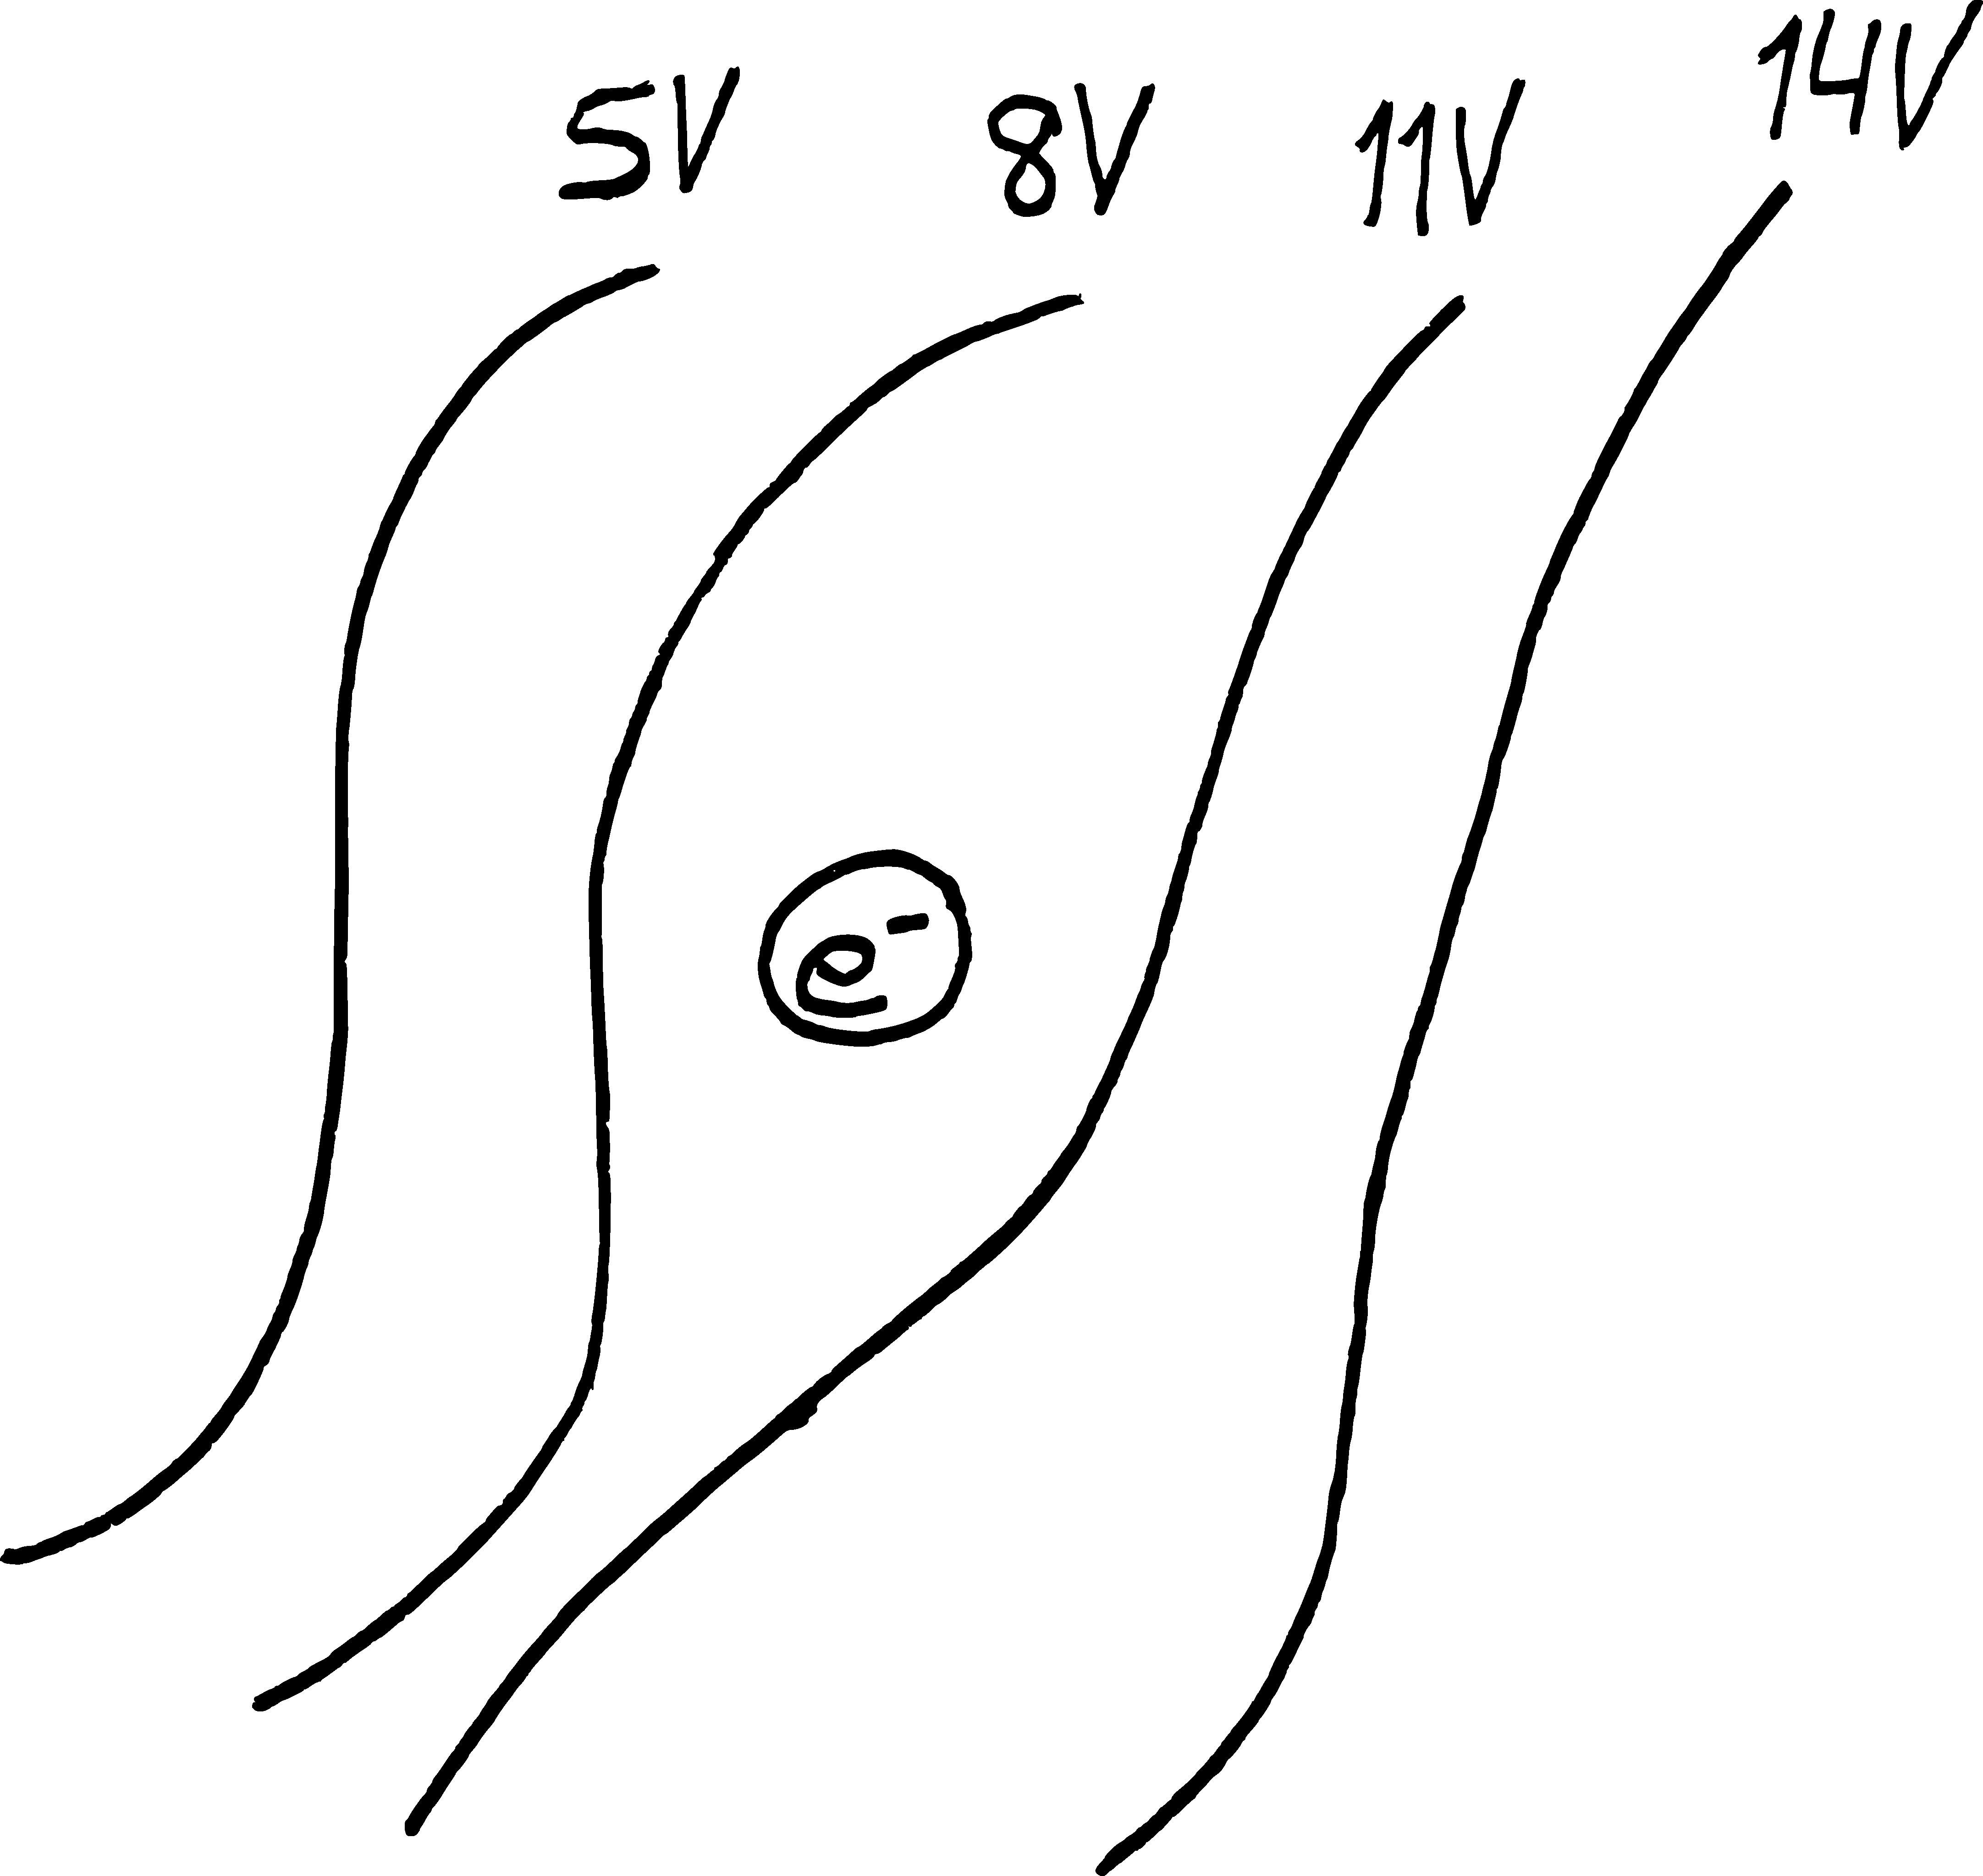
\includegraphics[width=5cm]{04-potentiel/figures/exercice-equipotentielles.pdf}
  \end{center}

  \begin{enumerate}
    \item Dans quelle direction est la force que subit l'électron?
    \item Tracez les lignes de champ électrique.
  \end{enumerate}
\end{diapobox}

\begin{reponsebox}
  \begin{center}
    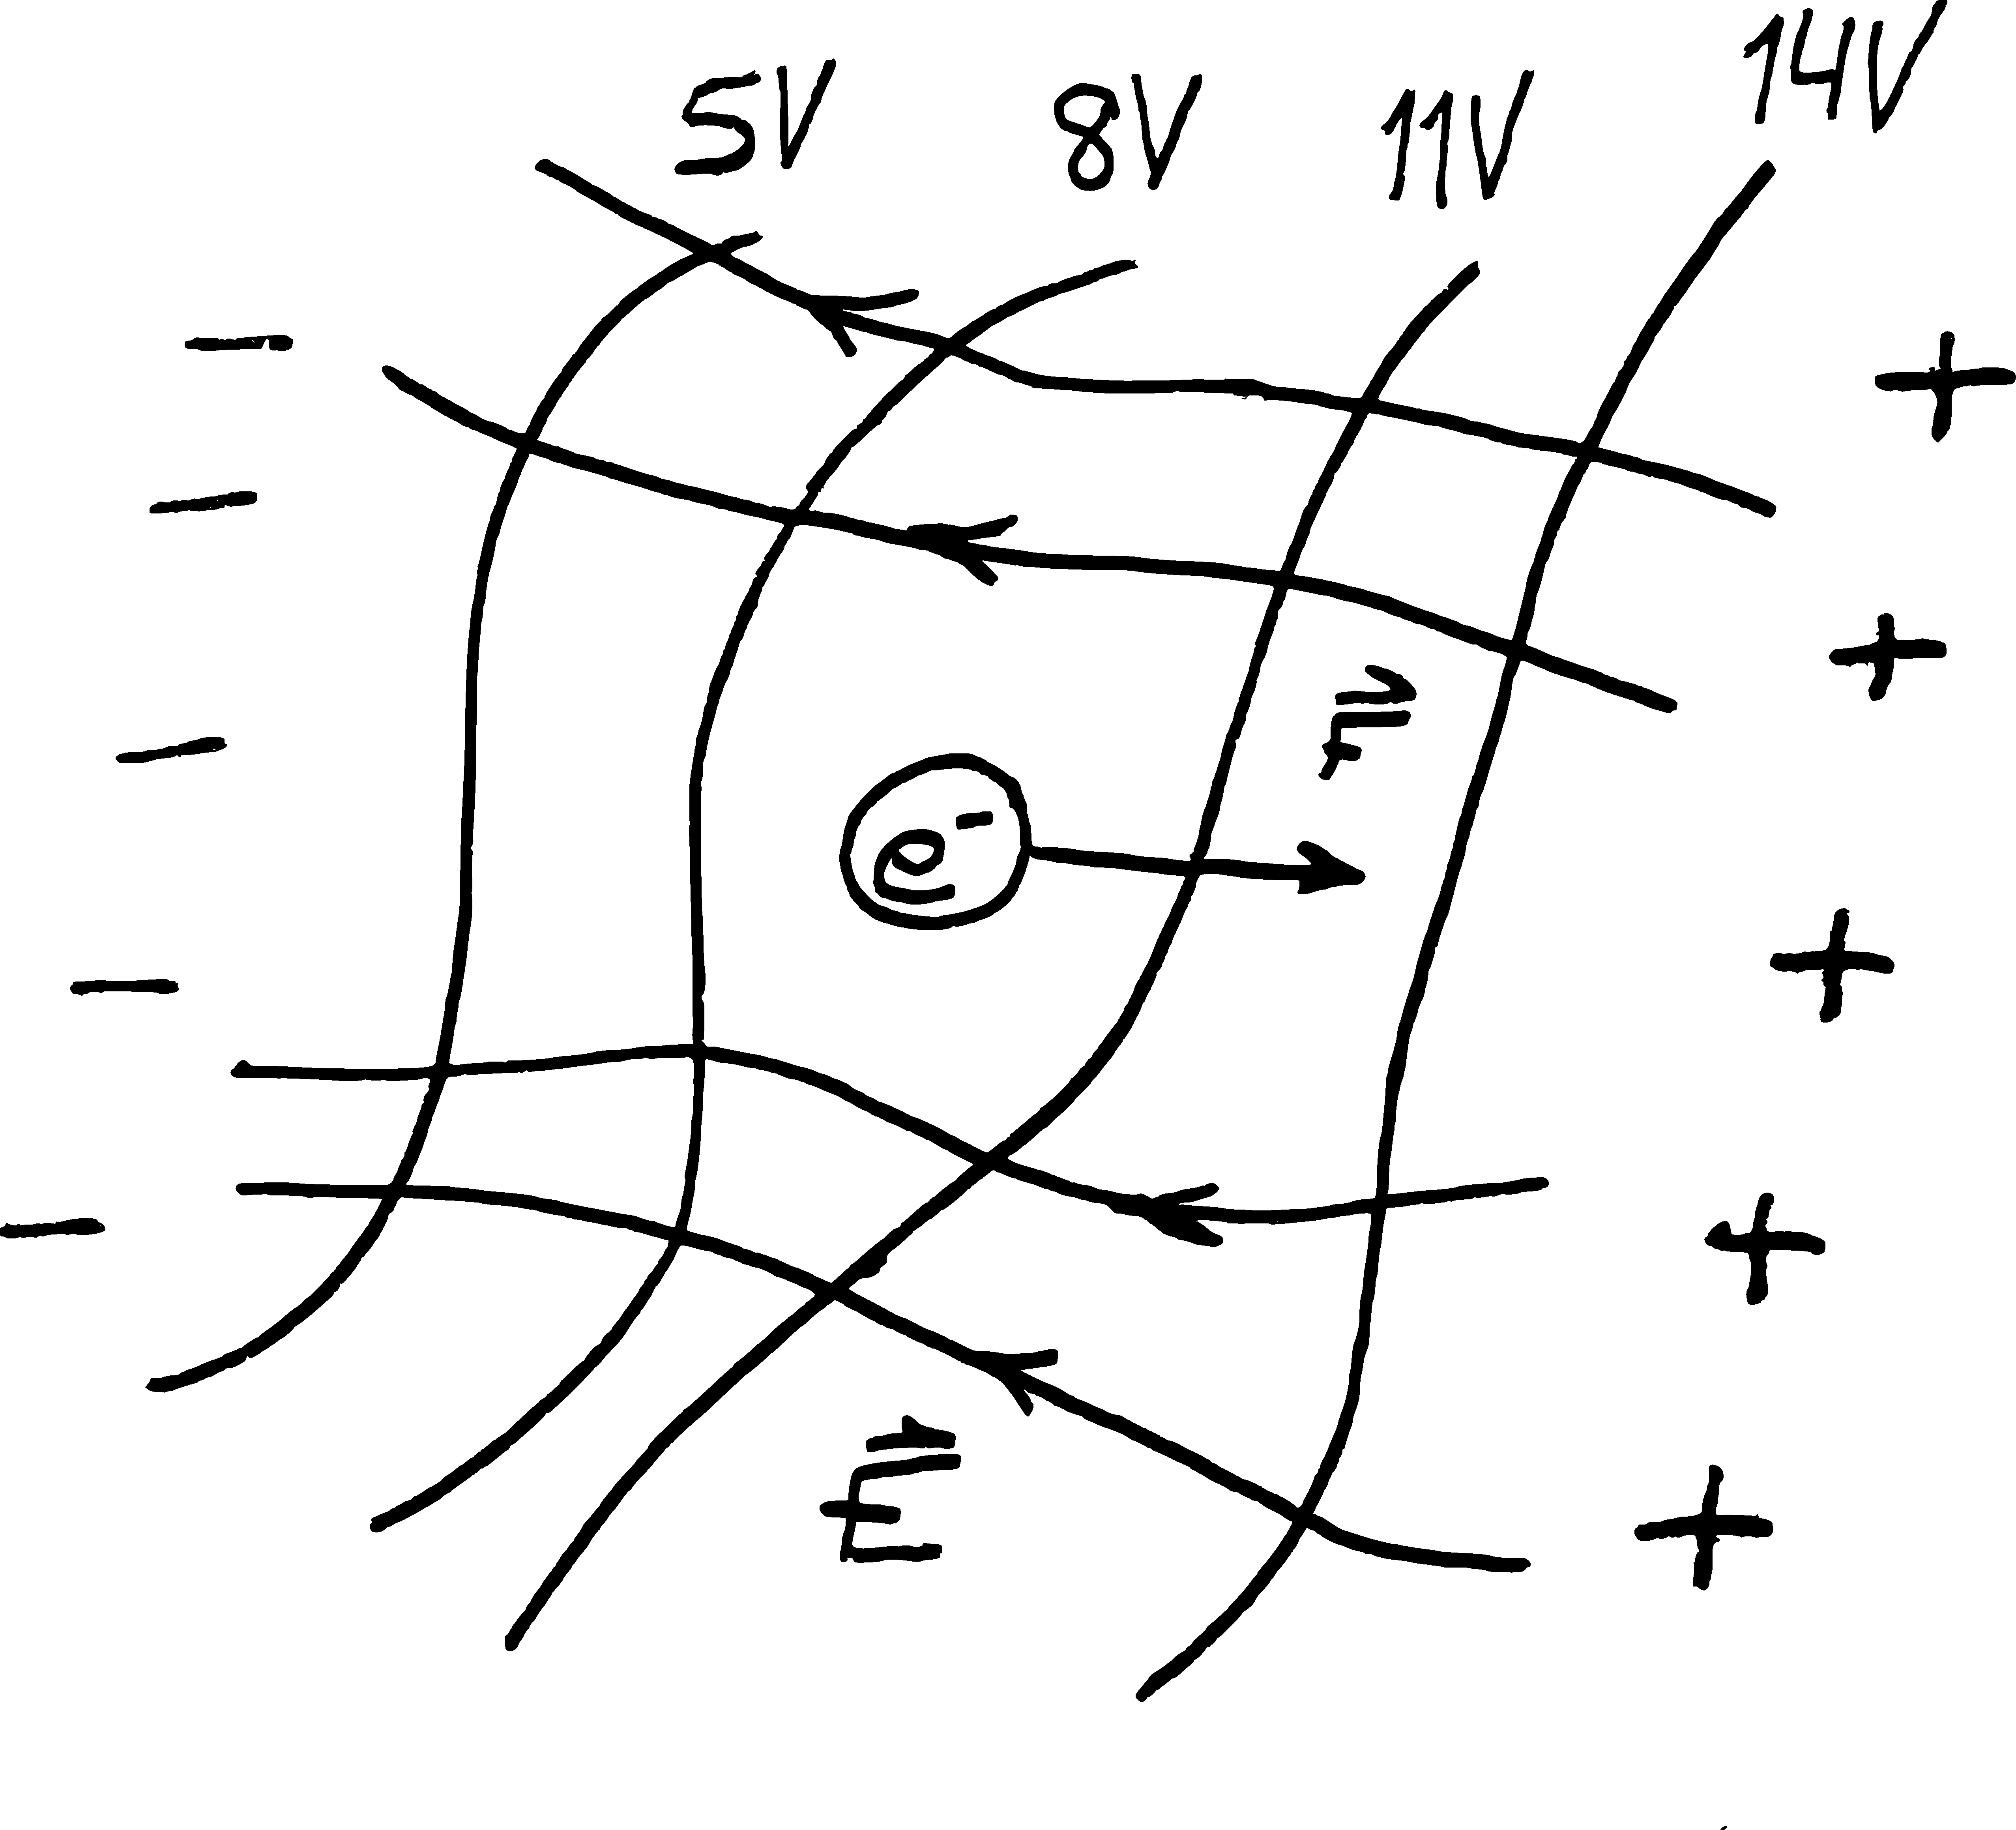
\includegraphics[width=5cm]{04-potentiel/figures/exercice-equipotentielles-solution.pdf}
  \end{center}
\end{reponsebox}


Cet exercice permet de mettre en lumière quelques propriétés importantes des
équipotentielles et du potentiel électrique.

\begin{itemize}
  \item Plus les équipotentielles sont rapprochées les unes des autres, plus le
    champ électrique est grand à cet endroit.
  \item Les lignes de champ électrique vont des potentiels élevés vers les
    potentiels faibles.
  \item Une particule chargée négativement subira une force vers les potentiels
    élevés.
  \item Une particule chargée positivement subira une force vers les potentiels
    plus faibles.
\end{itemize}



\section{Potentiel électrique d'une charge ponctuelle}

\marginnote{
  Lafrance \S 4.4
}

Pour une charge ponctuelle
\[
  E_r = \coulombcst \frac{q}{r^2}.
\]
La différence de potentiel entre deux points $A$ et $B$ est donc
\begin{align*}
  \Delta V &= -\int_A^B \vec{E}\cdot d\vec{s} \\
    &= -\int_{r_A}^{r_B} \coulombcst \frac{q}{r^2} \,dr \\
    &= -kq \int_{r_A}^{r_B} \frac{1}{r^2} \,dr \\
    &= -kq \left[ \frac{-1}{r} \right]_{r_A}^{r_B} \\
    &= \frac{kq}{r_B} - \frac{kq}{r_A} \\
    &= V_B - V_A
\end{align*}
donc
$$V = \frac{kq}{r}$$



\section{Potentiel d'un ensemble de charges}

\marginpar{
  Tremblay \S 4.3

  Lafrance \S 4.5
}

\begin{fondamentalbox}
Le principe de superposition s'applique au potentiel électrique :
le potentiel d'un ensemble de charges est la somme des potentiels.
\end{fondamentalbox}

On peut utiliser ce principe pour calculer le potentiel de n'importe quel objet
chargé :
\[
  V = \int_\text{objet} \frac{k dq}{r}.
\]


\minisec{Énergie potentielle électrique d'un ensemble de charges}

On considère un ensemble de $n$ charges ponctuelles $q_1, q_2, \ldots, q_n$.
Pour calculer l'énergie potentielle de cet ensemble de charges, on doit
l'assembler, une charge à la fois. Placer la première charge ne requiert aucun
travail puisque le champ électrique est nul au départ. Apporter la seconde
charge nécessite un travail puisqu'on doit la déplacer dans le champ électrique
produit par la première charge. L'énergie requise est
\[
  U_2 = q_2 V_1.
\]
Pour la troisième charge, on doit tenir compte du potentiel créé par les deux
premières charges. Puisque le potentiel respecte le principe de superposition,
on a
\[
  U_3 = q_3 V_1 + q_3 V_2 = q_3 (V_1 + V_2).
\]
On peut répéter l'argument pour les charges suivantes. On obtient l'énergie
potentielle totale du système en additionnant les énergies $U_1, U_2, \ldots,
U_n$.  La somme contient un terme pour chaque paire de charges.
\[
  U = \sum_{i < j} q_i V_j
\]


\begin{diapobox}

  \minisec{Exercice}

  Trois charges sont placées aux sommets d'un carré de côté $d = \SI{3}{cm}$. Les
  charges sont de $q_1 = \SI{1.7}{\micro\coulomb}$, $q_2 = \SI{-3}{\micro\coulomb}$,
  et $q_3 = \SI{2}{\micro\coulomb}$.

  \begin{itemize}
    \item Déterminer le potentiel au point $P$, \SI{3}{cm} au-dessus de la
      charge $q_1$.
    \item On amène une charge $q_4 = \SI{-4}{\micro\coulomb}$ de l'infini jusqu'à $P$.
      Quel est le changement d'énergie potentielle du système? Que signifie la
      réponse?
  \end{itemize}

  \begin{center}
    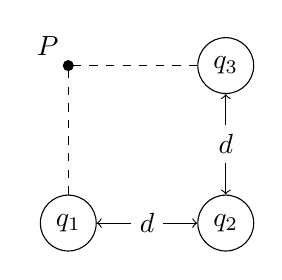
\begin{tikzpicture}
      \coordinate (p1) at (0, 0);
      \coordinate (p2) at (2, 0);
      \coordinate (p3) at (2, 2);
      \coordinate (p4) at (0, 2);
      \node[draw, circle] (q1) at (p1) {$q_1$};
      \node[draw, circle] (q2) at (p2) {$q_2$};
      \node[draw, circle] (q3) at (p3) {$q_3$};
      %\node[draw, circle] (q4) at (p4) {$q_4$};
      \fill (p4) circle (2pt);
      \node[anchor=south east] at (p4) {$P$};
      \draw[<->] (q1) -- node[fill=white] {$d$} (q2);
      \draw[<->] (q2) -- node[fill=white] {$d$} (q3);
      \draw[dashed] (q1) -- (p4);
      \draw[dashed] (q3) -- (p4);
    \end{tikzpicture}
  \end{center}
\end{diapobox}

\begin{reponsebox}
  \begin{align*}
    V &= V_1 + V_2 + V_3 \\
      &= \frac{kq_1}{r_1} + \frac{kq_2}{r_2} + \frac{kq_3}{r_3} \\
      &= \SI{509433}{V} + \SI{-635689}{V} + \SI{599333}{V}  \\
      &= \SI{473078}{V}
  \end{align*}

  Le potentiel à l'infini est nul donc $\Delta U = U_f - U_i = U_f$.
  \begin{align*}
    U &= q_4 (V_1 + V_2 + V_3)  \\
      &= \SI{-1.89}{J}
  \end{align*}
  L'énergie potentielle du système a diminué, ce qui signifie que le système
  est plus stable dans cette configuration que lorsque la charge $q_4$ est à
  l'infini.
\end{reponsebox}
